\documentclass[a4paper,conference]{IEEEtran}
\IEEEoverridecommandlockouts

\usepackage{cite}
\usepackage{amsmath,amssymb,amsfonts}
\usepackage{textcomp}
\usepackage{url}
\usepackage{array}
\usepackage{balance}
\usepackage{tikz}
\usepackage{graphicx}
\usepackage[table]{xcolor}
\usetikzlibrary{positioning,arrows.meta,calc}

% ICAC 2026 uses double blind review. Keep this true for the review submission.
% Set it to false only for the camera ready paper after acceptance.
\newif\ificacblind
\icacblindtrue

\def\BibTeX{{\rm B\kern-.05em{\sc i\kern-.025em b}\kern-.08em
    T\kern-.1667em\lower.7ex\hbox{E}\kern-.125emX}}

\begin{document}

\title{SinhalaJournal-LLM: Data Centric Adaptation of a Sinhala Language Model for Journalism}
\newcommand{\systemname}{SinhalaJournal-LLM}

\author{}

\maketitle

\begin{abstract}
Sinhala has limited Natural Language Processing (NLP) support for practical
newsroom writing. This research presents \systemname, which adapts SinLlama
for grammar correction, headline generation, news summarization, and style
rewriting using separate Low Rank Adaptation (LoRA) adapters. From 1,031,456
collected Sinhala news articles, quality filtering retained 665,887. On a
frozen and manually reviewed grammar benchmark of 286 inputs, the v27 adapter
achieved 56.99\% overall exact match and corrected 63 of 143 faulty sentences.
ByT5-small corrected 12 faulty sentences and mT5-small corrected none. A
rescoring of saved v24 and v26 predictions shows that exact match against the
repaired gold increases from 57.8\% to 65.6\%. On the stricter 143 case subset
where the gold is unchanged and both models receive identical inputs, exact
match increases from 61.5\% to 66.4\%. This indicates broader correction gains
as well as better agreement with the repaired convention. In headline
generation, balancing categories before splitting increased ROUGE-1 from
0.1382 to 0.2933 because duplicated articles entered both partitions. The
final v19 adapter reached ROUGE-1 of 0.1824 on 100 articles from an external
publisher. A later audit found about 81\% contamination in the legacy
summarization evaluation. After rebuilding the split at article level, the v06
and v07 recipes were effectively tied on 273 held out articles across three
length bands. Style target generation also showed serious template repetition
and copying. Only 7,555 of 22,236 candidates passed the final quality filters.
Overall, the results show that dataset construction, contamination control, and
evaluation design can strongly affect the measured performance of Sinhala
generative models.
\end{abstract}

\begin{IEEEkeywords}
Sinhala NLP, low resource language, LoRA, journalism NLP, data quality
\end{IEEEkeywords}

\section{Introduction}
Large Language Models (LLMs) have improved text generation, but Sinhala still has
fewer datasets, benchmarks, and systems for specific tasks
\cite{desilva2019survey,jayakody2024performance}. SinBERT established strong
Sinhala text classification baselines \cite{dhananjaya2022bertifying}, while
SinLlama extended Llama 3 with Sinhala vocabulary and continual pretraining
\cite{grattafiori2024llama3,aravinda2025sinllama}. NSina later provided a large
Sinhala news corpus and headline generation benchmark
\cite{hettiarachchi2024nsina}.

Journalism needs several forms of constrained generation. Editors correct
language, write headlines under length limits, condense reports, and adapt the
same facts to different editorial styles. Names, numbers, dates, quotations,
and meaning must remain correct during these operations. Sinhala studies have
addressed individual tasks such as extractive summarization
\cite{jahan2023summarization} and rule based spelling and grammar correction
\cite{goonawardena2022grammar}. However, adapting one Sinhala decoder across
these connected newsroom tasks remains less explored.

\systemname{} uses SinLlama as a shared base and trains one LoRA adapter
\cite{hu2022lora} for each task. The base is loaded in 4 bit form so repeated
adaptation remains practical on limited hardware \cite{dettmers2023qlora}.
The study contributes four task datasets derived from an original news corpus
and evaluates a separate adapter for each task. It also provides a frozen
grammar comparison with ByT5-small and mT5-small, a grammar safety policy
replay, a measured case of headline split leakage, and Sinhala data quality
findings related to Unicode handling, summarization decoding, and template
repetition in style rewriting. The study focuses on how data and evaluation
choices change the measured quality of a low resource generative system.

\section{Related Work}

\subsection{Sinhala Language Models and Generation Tasks}
Sinhala NLP has progressed from rule based processing to pretrained models.
SinBERT and later Sinhala encoder models improved representation and
classification \cite{dhananjaya2022bertifying,ranasinghe2025encoder}, but are
not generative decoders. SinLlama is the closest foundation for this work.
It extends Llama 3 8B with Sinhala vocabulary and continual pretraining, then
uses LoRA for downstream classification \cite{aravinda2025sinllama}. Our work
instead studies constrained generation from the same type of decoder adapted for Sinhala.

NSina contains over 500,000 Sinhala news articles and benchmarks media
identification, category prediction, and headline generation
\cite{hettiarachchi2024nsina}. Sinhala summarization work has compared TF-IDF
and TextRank \cite{jahan2023summarization}, while multilingual sequence to sequence models such as mT5 and XL-Sum support abstractive generation
\cite{xue2021mt5,hasan2021xlsum}. Existing Sinhala spelling and grammar systems include rule based and hybrid
approaches \cite{goonawardena2022grammar}.
These studies provide useful baselines for individual tasks but do not evaluate the four
connected editorial operations together.

\subsection{Adaptation and Evaluation of Constrained Generation}
LoRA freezes the pretrained weights and learns low rank updates, while QLoRA
combines adapter training with a quantized base model
\cite{hu2022lora,dettmers2023qlora}. This makes separate adapters feasible
without maintaining four full 8B models. Evaluation remains task dependent.
Style transfer, for example, must balance style change, content preservation,
and fluency, for which overlap metrics alone are inadequate
\cite{ostheimer2024tst}. For this reason, each task is evaluated with measures suited to its own objective.

\section{Corpus and Task Datasets}
Project crawlers and scraping scripts collected 1,031,456 articles directly
from Sri Lankan Sinhala news sites, spanning 13 March 2008 to 4 March 2026. No
NSina data were used. Exact duplicates were removed, after which articles were
accepted only when the body contained between 300 and 10,000 characters, the title
contained between 10 and 200 characters, and at least 30\% of the characters were Sinhala Unicode. Failed rows
were discarded rather than truncated. The process removed 365,569 articles
(35.4\%), leaving 665,887. Local news and Politics were the largest categories,
with 264,434 and 151,640 articles respectively, followed by International
(68,005), Business (49,247), Sports (37,336), and Editorial (16,263). The
remaining 78,962 articles were distributed across Other, Entertainment,
Crime/Law, Health, Technology, Science, Religion, and Environment. This
distribution matters for generation experiments because the categories are
highly uneven. This can make simple category balancing
appear useful even when it creates the leakage problem demonstrated later.

\subsection{Invisible Character Handling}
Sinhala scraping exposed two visually similar characters that require different
treatment. Soft hyphen U+00AD is invisible but disrupts subword tokenization and
is removed. It appeared in 85.8\% of the rows in one style working file.
Zero width joiner U+200D participates in valid Sinhala conjuncts and is
preserved. We also observed encoding artifacts and a Devanagari danda attached
to surrounding text without whitespace in 480 of 600 inspected rows, which
broke downstream sentence splitting. The practical finding is that generic
removal of invisible or control characters can corrupt Sinhala text, so
normalization must be character aware.

\subsection{Task Datasets}
None of the tasks uses the full corpus. Each dataset was independently filtered,
transformed, and audited, as summarized in Table~\ref{tab:datasets}.

\begin{table}[!b]
\caption{Final task datasets used for adapter development}
\label{tab:datasets}
\centering
\footnotesize
\setlength{\tabcolsep}{2.6pt}
\renewcommand{\arraystretch}{1.05}
\begin{tabular}{|p{0.17\columnwidth}|p{0.25\columnwidth}|p{0.45\columnwidth}|}
\hline
\textbf{Task} & \textbf{Final data} & \textbf{Main structure} \\
\hline
Grammar & 36,006 rows & Incorrect or correct input with corrected target \\
\hline
Headline & 43,737 train, about 4,795 validation & Article, category, reference headline \\
\hline
Summary & 35,547 articles & Article with short, medium, and long summaries \\
\hline
Style & 7,555 rewrites & Article, target style, rewritten article \\
\hline
\end{tabular}
\end{table}

The summary row reports the cleaned v07 dataset. The tracked v06 model was
trained before the 22-row cleanup on 35,569 articles.

\textit{Grammar.} The final Stage 13 file contains 36,006 rows spanning
spelling, verb form, agreement, word order, spacing, register, pronouns,
negation, numerals, and already correct controls. Stage 12 and Stage 13 contain
the same 36,006 inputs in the same order, while 4,999 target outputs differ.
The training data combine manually curated material with controlled
corpus derived error construction and preservation cases.

\textit{Headline.} The final v19 training set contains 43,737 rows with short
(3--5 words), medium (6--7), and long (8--10) target bands. Earlier category
balancing physically duplicated minority examples before splitting, which
created the leakage quantified in Section~VI-B. Later target cleaning removes
media and scraper artifacts.

\textit{Summarization.} The v06 silver corpus contains 35,569
articles, each paired with short, medium, and long summaries. A quality audit
removed 22 rows with joined word or numeric unit defects, producing the 35,547 row
v07 cleaned corpus. The legacy scripts expanded the three length variants
before splitting, which later proved to contaminate evaluation. A deterministic
article level 80/10/10 split was therefore frozen from the raw corpus: 28,455
training, 3,556 validation, and 3,558 test articles, plus a fixed 300 article
evaluation subset. Both v06 and v07 recipes were retrained on these boundaries.

\textit{Style rewriting.} The final cleaned dataset contains 7,555 rewrites
across formal news, editorial, sports, youth, and feature styles. It was
retained from 22,236 generated candidates after structural, factual, script,
length, repetition, and copying checks. Earlier target files exhibited severe
verbatim copying and repeated template behavior, motivating regeneration and
filtering before v13 training.

\section{Model Adaptation and Fine Tuning}

\subsection{Base Model}
SinLlama is the common base. We begin from the model already adapted for Sinhala rather than
repeating its tokenizer extension or continual pretraining
\cite{aravinda2025sinllama}. The merged checkpoint is loaded in 4 bit NF4 with
BF16 compute, and each task uses a separate LoRA adapter. Fig.~\ref{fig:modeladaptation}
summarizes the relationship.

\begin{figure}[!t]
\centering
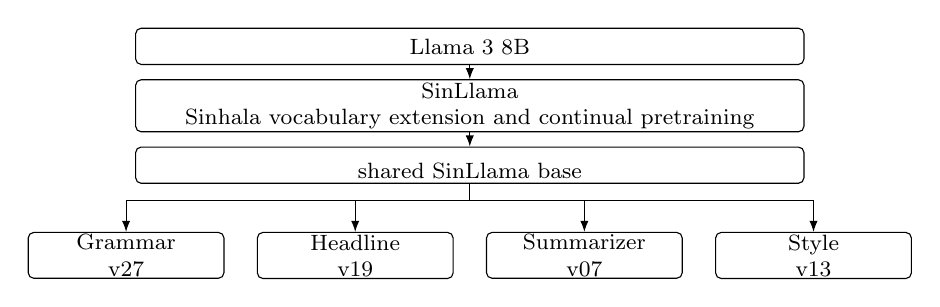
\begin{tikzpicture}[
    base/.style={draw, rounded corners=2pt, align=center,
        minimum width=0.70\columnwidth, minimum height=4.6mm,
        inner sep=1.1pt, font=\footnotesize},
    adapter/.style={draw, rounded corners=2pt, align=center,
        minimum width=0.205\columnwidth, minimum height=4.8mm,
        inner sep=0.8pt, font=\footnotesize},
    flow/.style={-{Latex[length=1.4mm]}, line width=0.4pt},
    branchline/.style={line width=0.4pt}
]
\node[base] (llama) {Llama 3 8B};
\node[base, below=1.8mm of llama] (sinllama)
    {SinLlama\\Sinhala vocabulary extension and continual pretraining};
\node[base, below=1.8mm of sinllama] (shared)
    {\systemname{}\\shared SinLlama base};

\node[adapter, below=6.1mm of shared, xshift=-0.36\columnwidth] (grammar)
    {Grammar\\v27};
\node[adapter, below=6.1mm of shared, xshift=-0.12\columnwidth] (headline)
    {Headline\\v19};
\node[adapter, below=6.1mm of shared, xshift=0.12\columnwidth] (summary)
    {Summarizer\\v07};
\node[adapter, below=6.1mm of shared, xshift=0.36\columnwidth] (style)
    {Style\\v13};

\draw[flow] (llama) -- (sinllama);
\draw[flow] (sinllama) -- (shared);
\coordinate (branch) at ($(shared.south)+(0,-2.1mm)$);
\coordinate (gbranch) at (grammar.north |- branch);
\coordinate (hbranch) at (headline.north |- branch);
\coordinate (sbranch) at (summary.north |- branch);
\coordinate (tbranch) at (style.north |- branch);
\draw[branchline] (shared.south) -- (branch);
\draw[branchline] (gbranch) -- (tbranch);
\draw[flow] (gbranch) -- (grammar.north);
\draw[flow] (hbranch) -- (headline.north);
\draw[flow] (sbranch) -- (summary.north);
\draw[flow] (tbranch) -- (style.north);
\end{tikzpicture}
\caption{Model adaptation architecture of \systemname{}.}
\label{fig:modeladaptation}
\end{figure}

\subsection{Prompt Design}
Prompts encode the constraints later evaluated. Grammar instructs the model to
fix only errors and return correct text unchanged. Headline prompts include
category and requested word band. Summarization uses instructions for each requested length that restrict content to the source. Style uses a target style
instruction with factual preservation rules for entities, numbers, dates,
quotations, honorifics, and unsupported substitutions. We therefore treat the
prompt as part of the task definition rather than only an interface wrapper.

\subsection{LoRA Configuration}
All adapters target the same seven attention and MLP projections and use seed
42 with validation loss checkpoint selection. Table~\ref{tab:config} records
the selected configurations. Grammar v27 is a lower rank and lower scaling
configuration ($r=4,\alpha=4$) rather than a pure rank only ablation. The
leakage controlled summarization comparison retrains both the raw v06 and
cleaned v07 recipes with the same $r=32,\alpha=64$ configuration on frozen
article level boundaries.

\begin{table*}[!t]
\caption{Selected LoRA configurations. All use a 4 bit NF4 SinLlama base with BF16 compute and the same seven target projections.}
\label{tab:config}
\centering
\footnotesize
\setlength{\tabcolsep}{4pt}
\renewcommand{\arraystretch}{1.08}
\begin{tabular}{|l|l|r|c|r|c|c|c|r|}
\hline
\textbf{Task} & \textbf{Adapter/recipe} & \textbf{Train data} & \textbf{$r$\,/\,$\alpha$\,/\,dropout} &
\textbf{Max seq.} & \textbf{Eff. batch} & \textbf{LR} & \textbf{Epochs} & \textbf{Trainable params} \\
\hline
Grammar       & v27 & 36,006 rows & 4\,/\,4\,/\,0.05    & 512  & 8  & 5e-5 & 3.00  & 10,485,760 \\
\hline
Headline      & v19 & 43,737 rows & 64\,/\,128\,/\,0.08 & 768  & 8  & 5e-5 & 8 (early stop) & 167,772,160 \\
\hline
Summarization & v06/v07 frozen & 28,455 articles & 32\,/\,64\,/\,0.05  & 2048 & 16 & 2e-4 & 3 & 83,886,080 \\
\hline
Style         & v13 & 7,555 rows  & 24\,/\,48\,/\,0.05  & 4096 & 16 & 1e-4 & 3 & 62,914,560 \\
\hline
\end{tabular}
\end{table*}

\subsection{Inference Configuration}
Grammar and style use deterministic decoding. Headline generation samples at
temperature 0.3 and top-$p$ 0.9 with a retry when the first output is too short. Summarization uses
deterministic decoding and separate token limits for each requested length. An earlier
\texttt{no\_repeat\_ngram\_size=3} setting was removed after it corrupted
opening Sinhala grapheme sequences, showing that decoding constraints commonly
used for other languages are not automatically safe for Sinhala.

\textit{Reproducibility and data use.} Grammar v27 was trained on one NVIDIA
A40 for 6.36 hours with 44.352 GB peak GPU memory. The frozen summarization
retraining used the same GPU and persisted split manifests and result files.
The multiple length silver summaries used by v06/v07 were generated through the
project's local OpenAI compatible multi router gateway using
\texttt{ollama/gpt-oss:120b}, with quality validation and resume support. The
corpus came from publicly accessible news pages for academic research, and full
article text is not redistributed in this manuscript. Repository links are
omitted for double blind review.

\section{Evaluation Protocol}
Each task uses a different definition of correctness. Grammar Stage 6 is a
frozen and manually reviewed set of 286 unseen inputs. It contains 143 cases
that require correction and 143 paired controls that should remain unchanged.
The faulty cases include 55 natural errors found in published news text, 80
injected unseen orthography cases, and eight spacing or punctuation cases. No
normalized input appears in the final training data or Stage 5. In addition,
87 faulty cases contain exact correction pairs that do not occur in training.

Stage 6 reports overall exact match, exact match on faulty cases, clean
preservation, edit $F_{0.5}$, and recall on unseen correction pairs. Confidence
intervals are calculated with document clustered bootstrap sampling. The same
286 inputs are used for Grammar v25, Grammar v27, ByT5-small, and mT5-small.
The ByT5 and mT5 baselines use the frozen Stage 13 source with 28,519 training
cases and 1,518 development cases. Rare correction pairs remain disjoint and
330 bridge cases are excluded. Both baselines were trained for three epochs.
The mT5 safety layer rejected malformed outputs, so its applied Stage 6 result
is the same as the unchanged input baseline.

The Stages 2 to 5 benchmark contains 154 development examples. Saved v24 and
v26 predictions are rescored against both the original and repaired gold. Of
the 154 cases, 145 have unchanged gold and nine have changed gold. The
strictest comparison uses 143 cases where the gold did not change and both
models received byte identical inputs. The same development predictions are
used for the grammar validator replay.

Headline evaluation first compares the leaked split with the repaired split.
It then evaluates v18, v19, and v20 using 300 validation articles at all three
requested lengths, giving 900 outputs for each version. An output is marked as
an artifact when it contains prompt or media tags, truncation, empty text, or
content from another script. Final v19 is also evaluated on the same 100 Hiru
News articles previously used for v17.

For summarization, the older sample level split is compared with a frozen split
created at article level. The v06 and v07 recipes are then retrained using the
same training and validation boundaries. They are tested on a fixed subset of
300 articles. A total of 273 complete articles produce 819 generations for each
adapter. We report ROUGE-1, ROUGE-2, ROUGE-L, requested length adherence,
clean sentence ending, joined word defects, and numeric unit mismatch. The
compression ranges are 0.04 to 0.18 for short summaries, 0.12 to 0.32 for
medium summaries, and 0.22 to 0.55 for long summaries.

Style v13 uses a development diagnostic with 75 outputs and 15 examples for
each style. ROUGE is measured against reference rewrites, while copying is
checked against the source article. This set is not a frozen independent
benchmark and the production prompt differs from the training and evaluation
prompt. The results are therefore reported as development evidence rather than
final style accuracy.

\section{Results and Discussion}
\subsection{Grammar Correction}
Table~\ref{tab:grammar} reports Stage 6. v25 and v27 both correct 63 of 143
faulty inputs. v25 preserves one additional control. Their clustered 95\%
intervals overlap substantially, so the one example aggregate difference does
not establish superiority. v27 is retained for parameter efficiency because its
$r=4,\alpha=4$ adapter uses about one eighth of the trainable parameters of the
rank-32 configurations while remaining statistically comparable on Stage 6.

\begin{table}[!t]
\caption{Grammar Stage 6 comparison on 286 unseen inputs}
\label{tab:grammar}
\centering
\footnotesize
\setlength{\tabcolsep}{1.6pt}
\renewcommand{\arraystretch}{1.04}
\begin{tabular}{|l|r|r|r|r|}
\hline
\textbf{System} & \textbf{Overall} & \textbf{Change} & \textbf{$F_{0.5}$} & \textbf{Unseen} \\
\hline
Grammar v27 & 56.99\% & 44.06\% & 45.36\% & 40.23\% \\
\hline
Grammar v25 & 57.34\% & 44.06\% & 46.21\% & 41.38\% \\
\hline
ByT5-small & 50.00\% & 8.39\% & 20.34\% & 13.79\% \\
\hline
mT5-small & 50.00\% & 0.00\% & 0.00\% & 0.00\% \\
\hline
\end{tabular}
\end{table}

The 50\% overall floor is the unchanged input baseline because half of Stage 6
contains already correct controls. ByT5 repairs 12 faulty cases but also damages
12 controls. mT5's safety applied outputs exactly reproduce the unchanged
baseline. Under these evaluated formulations, the adapted SinLlama systems are
substantially better at making required corrections, although unseen pair
recall remains near 40\% and clean preservation near 70\%.

The two gold analysis in Table~\ref{tab:gdual} resolves an important
interpretation issue in the target repair experiment. Against repaired gold,
v24 to v26 improves by 7.8 percentage points. Against old gold, the difference
is only 1.9 points. However, on the 145 examples whose gold never changed, v26
still improves from 60.7\% to 65.5\%. Restricting further to 143 cases that also
gave both models byte identical inputs gives 61.5\% versus 66.4\%. Thus the
improvement is not solely target convention matching, but the full 7.8 percentage point
gain cannot be attributed causally to general correction quality alone.

\begin{table}[!t]
\caption{v24/v26 two gold development rescoring}
\label{tab:gdual}
\centering
\footnotesize
\setlength{\tabcolsep}{3pt}
\renewcommand{\arraystretch}{1.03}
\begin{tabular}{|l|r|r|r|}
\hline
\textbf{Model} & \textbf{Old gold} & \textbf{Repaired gold} & \textbf{Strict 143} \\
\hline
v24 & 59.7\% & 57.8\% & 61.5\% \\
\hline
v26 & 61.7\% & 65.6\% & 66.4\% \\
\hline
\end{tabular}
\end{table}

The lower rank and lower scaling v27 configuration reaches 66.9\% exact match on
the same development benchmark, with 91\% on taught pairs and 48\% on untaught
pairs. This supports parameter efficiency, not a pure rank only causal claim.

The grammar rule validator is evaluated by replaying the same 154 saved v27
predictions. Rules alone preserve clean text but correct none of the faulty
examples. A legacy blanket veto policy suppresses useful neural edits, while a
recalibrated selective policy restores neural exact match and recall and
removes the observed unsupported entity mutation without increasing number
errors. Because the policy was developed on this set, this is a validator
ablation rather than an independent benchmark.

\begin{table}[!b]
\caption{Grammar validator replay on 154 development examples}
\label{tab:hybrid}
\centering
\footnotesize
\setlength{\tabcolsep}{2.3pt}
\renewcommand{\arraystretch}{1.03}
\begin{tabular}{|l|r|r|r|}
\hline
\textbf{System} & \textbf{Exact} & \textbf{Edit recall} & \textbf{Unsup. entity} \\
\hline
Neural v27 & 66.88\% & 71.14\% & 0.65\% \\
\hline
Rules only & 24.68\% & 0.00\% & 0.00\% \\
\hline
Legacy hybrid & 57.14\% & 56.22\% & 0.00\% \\
\hline
Recalibrated hybrid & 66.88\% & 71.14\% & 0.00\% \\
\hline
\end{tabular}
\end{table}

\subsection{Category Balancing Introduced Leakage}
\label{sec:leak}
An early headline dataset balanced minority categories by physical duplication
before the training and validation split. Copies of the same article therefore entered
both partitions. The leaked evaluation reported ROUGE-1 of 0.2933 and 485 exact
matches among 6,732 outputs, while the repaired split reported 0.1382 and no
exact matches among 4,795 outputs.

\begin{table}[!b]
\caption{ROUGE-1 for selected categories before and after repairing the split. Duplication factor is the upsampled validation count divided by the genuine count. }
\label{tab:leak}
\centering
\footnotesize
\setlength{\tabcolsep}{3pt}
\renewcommand{\arraystretch}{1.04}
\begin{tabular}{|l|r|r|r|r|}
\hline
\textbf{Category} & \textbf{Genuine $n$} & \textbf{Dup.} & \textbf{Leaked} & \textbf{Repaired} \\
\hline
\rowcolor{gray!10}
\textbf{Technology} & \textbf{10} & \textbf{40.0$\times$} & \textbf{0.7275} & \textbf{0.1320} \\
\hline
Human Rights  & 14  & 28.6$\times$ & 0.6295 & 0.0562 \\
\hline
Health        & 48  & 8.3$\times$  & 0.6044 & 0.1467 \\
\hline
Science       & 75  & 5.3$\times$  & 0.4843 & 0.1014 \\
\hline
Editorial     & 86  & 4.7$\times$  & 0.6339 & 0.0338 \\
\hline
Law and Order & 230 & 1.7$\times$  & 0.2422 & 0.1157 \\
\hline
Sports        & 722 & 1.0$\times$  & 0.1713 & 0.1646 \\
\hline
Politics      & 722 & 1.0$\times$  & 0.1502 & 0.1292 \\
\hline
\end{tabular}
\end{table}

Table~\ref{tab:leak} makes the mechanism visible. Technology had only ten
genuine validation articles, was duplicated 40 times and reached 0.7275.
Sports and Politics required no duplication and changed comparatively little. Their remaining differences reflect the rebuilt validation composition after the split was reconstructed.
The practical lesson is to split before balancing and to report genuine
category counts together with scores. The combination of a very small genuine count
and an unusually high score exposed the fault.
The overall ROUGE value alone did not show the problem. Style training consequently uses weighted
sampling rather than duplicated rows, preserving the minority style sampling
probability without creating identical articles on both sides of its split.

\subsection{Headline Generation}
Table~\ref{tab:headline} compares the three requested headline lengths after
leakage repair. v18 has the highest overall band accuracy but 11.2\% of outputs
contain media artifacts. Cleaning target headlines in v19 reduces artifacts to
1.1\% while maintaining 79.7\% band accuracy. v20 additionally cleans article
inputs, but its evaluation inputs are already clean, so the test cannot isolate
that hypothesis. v19 is therefore retained as the best documented balance between the two measures.

\begin{table}[!t]
\caption{Headline results across 900 outputs per version using requested band accuracy and artifact rate}
\label{tab:headline}
\centering
\footnotesize
\setlength{\tabcolsep}{2.1pt}
\renewcommand{\arraystretch}{1.04}
\begin{tabular}{|l|c|c|c|c|c|}
\hline
\textbf{Ver.} & \textbf{Short} & \textbf{Medium} & \textbf{Long} & \textbf{Overall} & \textbf{R-1 / R-L} \\
\hline
v18 & 88.7 / 0.3 & 76.0 / 11.0 & 78.0 / 22.3 & 80.9 / 11.2 & 0.124 / 0.121 \\
\hline
\textbf{v19} & 89.7 / \textbf{0.0} & 74.3 / 0.3 & 75.0 / 3.0 & 79.7 / \textbf{1.1} & 0.134 / 0.130 \\
\hline
v20 & 84.7 / 0.3 & 75.3 / 1.0 & 79.7 / 2.3 & 79.9 / 1.2 & 0.139 / 0.136 \\
\hline
\end{tabular}
\end{table}

Final v19 was also rerun on the same 100 Hiru News articles previously used
for v17. ROUGE-1 improves from 0.1567 to 0.1824, ROUGE-2 from 0.0281 to
0.0472, and ROUGE-L from 0.1521 to 0.1794. BLEU becomes 0.0100 and one exact
match is observed. The average generated/reference length ratio is 0.716,
showing that cross publisher transfer remains lexically stronger than v17 but
continues to favor shorter headlines than the external house style.

\subsection{Style Rewriting and Synthetic Target Quality}
Early style target generation showed a problem in the synthetic target
distribution. Many targets copied the source article or reused the same style
templates. Increasing the amount of synthetic generation by more than five
times did not solve this problem. The targets were therefore regenerated and
filtered for copying, repetition, factual consistency, structure, script, and
length. Only 7,555 of 22,236 candidates (34.0\%) passed the final pipeline.

The v13 adapter has a development diagnostic containing 75 outputs with 15
examples for each style. Overall reference ROUGE-L is 0.784. It ranges from
0.730 for editorial to 0.892 for formal news, while the measured direct copy
rate is 0\%. These values show that the final pipeline no longer has the
original direct copying failure. However, they do not prove that every output
follows the requested style or preserves all facts. We therefore do not treat
source difference as evidence of semantic drift and do not present the custom
combined score as a standard style accuracy measure. A further test using the
production prompt is still needed because the serving prompt differs from the
prompt used for training and evaluation.

\subsection{News Summarization}
The summarization experiments compare extractive methods, multilingual sequence
to sequence models, and the adapted SinLlama decoder. Extractive methods such
as TextRank, KeyBERT, and TF-IDF select text directly from the article and
therefore avoid factual hallucination. They also run in under one millisecond
in the reported implementation. However, they cannot rewrite or compress
complex Sinhala clauses, so the outputs can read as disconnected sentence
selections. The mT5-base LoRA baseline was trained on the same silver data. In
our experiments it showed lower fluency and weaker semantic retention. One
likely reason is the fragmentation of Sinhala text under a generic
SentencePiece vocabulary. SinLlama uses a Sinhala extended vocabulary and
produced more natural abstractive outputs with direct control over summary
length.

The original v06 and v07 comparison used 15 corpus articles and three requested
lengths. A later audit reconstructed the training process and found that about
81\% of articles in the nominal held out set had already appeared in training
under another length variant. The original process first expanded each article
into short, medium, and long examples and then shuffled those examples before
splitting. An article stays completely outside training only when all three
variants enter the 15\% validation partition. The probability is
$P = 0.15^3 \approx 0.34\%$. Very high contamination is therefore the expected
result of this sample level split.

To remove this problem, we created an 80/10/10 split at article level and
retrained both the raw v06 recipe and the cleaned v07 recipe using the same
disjoint boundaries. The fixed evaluation subset contains 300 articles. A
total of 273 complete articles produced 819 summaries for each adapter.
Table~\ref{tab:summaryfrozen} shows that SinLlama follows the requested length
bands with 86.8\% to 94.1\% accuracy. More than 94\% of outputs also end
cleanly across all bands. These results are achieved without later truncation
or separate length prediction heads. ROUGE-L on the true held out data ranges
from 0.457 to 0.508.

The repaired evaluation also changes the interpretation of the v06 and v07
cleaning experiment. The two recipes are almost equal on clean held out data.
The largest ROUGE-L difference is only 0.0018 and length adherence changes by
small amounts in different directions. Both adapters have 0\% joined word
defects. Numeric unit mismatch stays below 1\% for every band. The earlier
small test that appeared to favor v06 was therefore affected by contamination
and should not be treated as evidence that cleaning reduced quality. Removing
the 22 defective teacher records adds protection against joined words and large
numeric scale errors without reducing lexical overlap. Entity factuality still
needs stronger evaluation because errors such as entity substitution are not
fully measured by ROUGE.

\begin{table}[!b]
\caption{Summarization evaluation on 273 held out articles (819 outputs per adapter)}
\label{tab:summaryfrozen}
\centering
\footnotesize
\setlength{\tabcolsep}{1.9pt}
\renewcommand{\arraystretch}{1.03}
\begin{tabular}{|l|cc|cc|cc|}
\hline
& \multicolumn{2}{c|}{\textbf{ROUGE-L}} & \multicolumn{2}{c|}{\textbf{In Band \%}} & \multicolumn{2}{c|}{\textbf{Clean End \%}} \\
\textbf{Length Band} & \textbf{v06} & \textbf{v07} & \textbf{v06} & \textbf{v07} & \textbf{v06} & \textbf{v07} \\
\hline
Short ($\sim$10\%)  & 0.5077 & 0.5077 & 93.4\% & 94.1\% & 98.5\% & 98.9\% \\
\hline
Medium ($\sim$20\%) & 0.4577 & 0.4559 & 92.7\% & 90.5\% & 95.2\% & 95.2\% \\
\hline
Long ($\sim$35\%)   & 0.4566 & 0.4575 & 86.8\% & 88.6\% & 94.9\% & 94.1\% \\
\hline
\end{tabular}
\end{table}

\section{System Integration}
The four tasks are available through web, browser, and Google Docs clients.
Requests go to a FastAPI backend that selects the required preprocessing and
LoRA adapter on the shared SinLlama server. Grammar can revert unsafe edits,
while headline output cleaning removes media tags. A combined system accuracy
is not reported because the four tasks have different objectives.

\section{Limitations and Future Work}
Evaluation strength differs across the four tasks. Grammar Stage 6 provides the
strongest frozen comparison, but it is based on local news and uses one project
review process rather than an independent study with multiple raters. Recall on
unseen correction pairs is also only about 40\%. The two gold development
analysis reduces the effect of repaired targets on interpretation, but it does
not make the v24 and v26 comparison a randomized causal experiment. All
adapters were trained with one fixed seed. Therefore, the bootstrap confidence
intervals measure uncertainty in the test set rather than variation across
repeated training runs.

Headline v19 has one test using an external publisher. The internal evaluator
also does not exactly reproduce the production prompt, which uses explicit
\texttt{Category:} and \texttt{Article:} fields. A direct NSina benchmark is
not reported, so this paper does not make a state of the art claim. The repaired
summarization evaluation now isolates articles and uses 273 held out articles.
However, automatic overlap measures and numeric unit checks do not fully
measure factual correctness of entities and events. Style rewriting has a 75
output development diagnostic rather than a frozen independent human benchmark.
Its training and evaluation prompt also differs from the serving prompt. Future
work will focus on testing the production prompts directly, stronger factuality
checks, and blind evaluation by multiple Sinhala journalism and language
experts.

\balance
\section{Conclusion}
\systemname{} adapts one shared Sinhala decoder to four newsroom tasks using
separate LoRA adapters. On frozen Grammar Stage 6, v27 corrects 63 of 143 faulty
inputs. ByT5-small corrects 12 and mT5-small corrects none under the tested
formulations. Rescoring with both the old and repaired gold shows two effects.
The model makes broader correction gains and also agrees more closely with the
repaired target convention. On the strict subset where the gold did not change
and the model inputs were identical, exact match increases from 61.5\% to
66.4\%. The much smaller grammar adapter with $r=4$ and $\alpha=4$ remains
comparable to rank 32 models. This supports parameter efficiency, but it does
not prove that rank alone caused the result.

The headline experiments show that duplication before splitting can more than
double the apparent ROUGE-1 score. Final v19 also improves over v17 on the same
100 articles from an external publisher. The style experiments show that more
synthetic data does not repair a poor target distribution by itself. Only
34.0\% of the final style candidates passed all quality filters. The
summarization audit found about 81\% contamination in the older evaluation.
After rebuilding the split at article level and retraining both recipes, v06
and v07 are almost equal on 273 held out articles. Across all four tasks, the
main finding is consistent. Target quality, clean data partitions, prompt
consistency, and correct evaluation should be checked before higher model
scores are treated as real progress.

\begin{thebibliography}{00}
\bibitem{desilva2019survey} N. de Silva, ``Survey on publicly available Sinhala natural language processing tools and research,'' arXiv:1906.02358, 2019.
\bibitem{jayakody2024performance} R. Jayakody and G. Dias, ``Performance of recent large language models for a low-resourced language,'' in \textit{Proc. Int. Conf. Asian Language Processing (IALP)}, 2024, pp. 162--167, doi: 10.1109/IALP63756.2024.10661169.
\bibitem{dhananjaya2022bertifying} V. Dhananjaya, P. Demotte, S. Ranathunga, and S. Jayasena, ``BERTifying Sinhala - a comprehensive analysis of pre-trained language models for Sinhala text classification,'' in \textit{Proc. LREC}, 2022, pp. 7377--7385.
\bibitem{grattafiori2024llama3} A. Grattafiori \textit{et al.}, ``The Llama 3 herd of models,'' arXiv:2407.21783, 2024.
\bibitem{aravinda2025sinllama} H. W. K. Aravinda \textit{et al.}, ``SinLlama - a large language model for Sinhala,'' in \textit{Proc. Moratuwa Eng. Res. Conf. (MERCon)}, 2025, pp. 617--622, doi: 10.1109/MERCon67903.2025.11217094.
\bibitem{hettiarachchi2024nsina} H. Hettiarachchi, D. Premasiri, L. Uyangodage, and T. Ranasinghe, ``NSina: A news corpus for Sinhala,'' in \textit{Proc. LREC-COLING}, 2024.
\bibitem{jahan2023summarization} M. A. C. Akmal Jahan and K. K. C. Wijesekara, ``Automated text summarization of Sinhala online articles,'' \textit{J. Science-FAS-SEUSL}, vol. 4, no. 1, pp. 1--15, 2023.
\bibitem{goonawardena2022grammar} M. Goonawardena, A. Kulatunga, R. Wickramasinghe, T. Weerasekara, H. De Silva, and S. Thelijjagoda, ``Automated spelling checker and grammatical error detection and correction model for Sinhala language,'' in \textit{Proc. Int. Res. Conf. Smart Computing and Systems Engineering (SCSE)}, 2022, pp. 184--189, doi: 10.1109/SCSE56529.2022.9905126.
\bibitem{hu2022lora} E. J. Hu \textit{et al.}, ``LoRA: Low-rank adaptation of large language models,'' in \textit{Proc. ICLR}, 2022.
\bibitem{dettmers2023qlora} T. Dettmers, A. Pagnoni, A. Holtzman, and L. Zettlemoyer, ``QLoRA: Efficient finetuning of quantized LLMs,'' in \textit{Advances in Neural Information Processing Systems}, 2023.
\bibitem{ranasinghe2025encoder} T. Ranasinghe \textit{et al.}, ``Sinhala encoder-only language models and evaluation,'' in \textit{Proc. 63rd ACL}, 2025, pp. 8623--8636.
\bibitem{xue2021mt5} L. Xue \textit{et al.}, ``mT5: A massively multilingual pre-trained text-to-text transformer,'' in \textit{Proc. NAACL-HLT}, 2021, pp. 483--498.
\bibitem{hasan2021xlsum} T. Hasan \textit{et al.}, ``XL-Sum: Large-scale multilingual abstractive summarization for 44 languages,'' in \textit{Findings of ACL-IJCNLP}, 2021, pp. 4693--4703.
\bibitem{ostheimer2024tst} P. S. Ostheimer, M. K. Nagda, M. Kloft, and S. Fellenz, ``Text style transfer evaluation using large language models,'' in \textit{Proc. LREC-COLING}, 2024, pp. 15802--15822.
\bibitem{xue2022byt5} L. Xue \textit{et al.}, ``ByT5: Towards a token-free future with pre-trained byte-to-byte models,'' \textit{Trans. Assoc. Comput. Linguistics}, vol. 10, pp. 291--306, 2022.
\bibitem{lin2004rouge} C.-Y. Lin, ``ROUGE: A package for automatic evaluation of summaries,'' in \textit{Text Summarization Branches Out}, 2004, pp. 74--81.
\end{thebibliography}

\end{document}
